\problemname{Waterfall}
Alexander likes water. Therefore, it's no surprise that he is fond of rushing water. This might
explain why he wants to create his own waterfall. Just imagine, water cascading endlessly!

He has found a cliff face that he believes will make the perfect waterfall after he adds some water.
The cliff face can be modeled as an $R \times C$ grid, where $N$ cells have an outcropping cliff.
Alexander plans to pour water from above so that it flows down in $K$ columns.

The water spreads in the grid according to the following rules: if the cell below the water is empty,
it spreads there. If there is a cliff in the way, it instead spreads to the right and left. If there
is a cliff in the way to the right or left, it does not spread in that direction. This also applies
to the water being poured from above, i.e., if water is poured into column $i$ and the top row has
a cliff in column $i$, it is as if water is also being poured from above in columns $i - 1$ and $i + 1$,
provided those columns are within the grid.

However, Alexander does not want to cause a flood because then all the water will stand still in the end.
Water that stands still is, of course, less exciting than rushing water. Therefore, he wants your help
to write a program that calculates how many columns have water in them in the bottom row of the cliff.

\begin{figure}[!h]
  \centering
  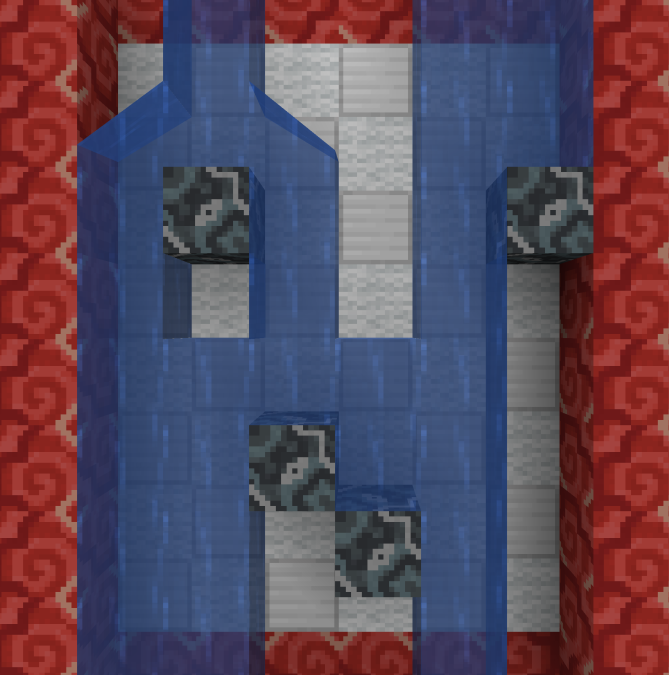
\includegraphics[width=7cm]{vatten1.png}
  \quad
  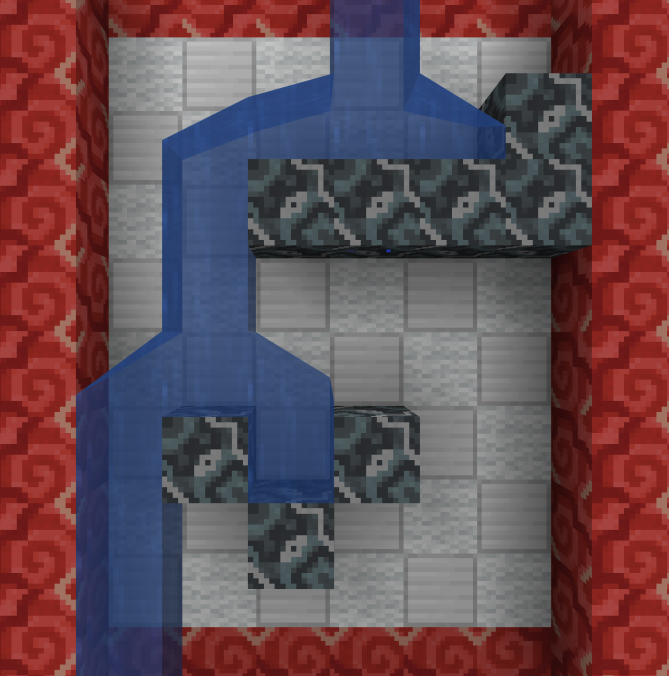
\includegraphics[width=7cm]{vatten2.png}
  \caption{An illustration of the flow in sample 1 and 2. The red frame marks the end of the cliff face.}
\end{figure}


\section*{Input}
The first line contains two integers $R, C$ ($1 \le R, C \le 10^9$), the number of rows and columns that make up the mountain.

The second line contains two integers $K, N$ ($1 \le K, N \le 10^5$), the number of columns with water and the number
of cliffs protruding from the mountain.

Following this are $K$ lines, where the $i$-th line contains a number $V_i$ ($0 \le V_i \le C-1$), indicating that water flows
down along column $V_i$ from above the grid. It is guaranteed that all $V_i$ are unique.

Afterward, there are $N$ lines where each line $i$ contains two integers $A_i$ ($1 \le A_i \le R-1$) and
$B_i$ ($0 \le B_i \le C-1$), representing the row and column where the $i$-th cliff is located.
These positions are also unique.

\section*{Output}
Print an integer: the number of columns that contain water in the bottom row of the grid.

\section*{Points}
Your solution will be tested on several test case groups.
To get the points for a group, it must pass all the test cases in the group.

\noindent
\begin{tabular}{| l | l | p{12cm} |}
  \hline
  \textbf{Group} & \textbf{Point value} & \textbf{Constraints} \\ \hline
  $1$    & $20$      & $R \cdot C \le 1000$ \\ \hline
  $2$    & $30$      & Cliffs can't touch each other diagonally, horizontally or vertically. \\ \hline
  $3$    & $20$      & Cliffs can't touch each other diagonally. \\ \hline
  $4$    & $30$      & No additional constraints. \\ \hline
\end{tabular}
